\section{Carte des vents}

\begin{questions}
	\question Les nombres sur la carte du document 1 correspondent à la valeur de la vitesse du vent en km/h et les flèches indiquent se direction et son sens dans les différentes villes.
	
	\question \ \\
		\begin{center}
			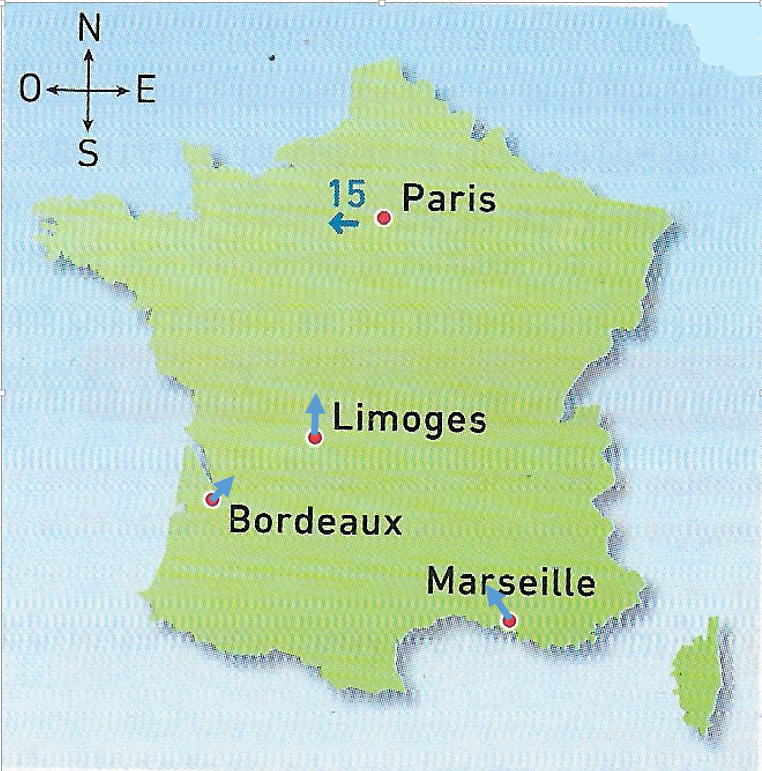
\includegraphics[scale=0.4]{carte2}
		\end{center}
		
	\question Le 23 octobre 2016, la valeur de la vitesse du vent est la même à Limoges et à Paris, mais leurs directions et leurs sens sont différents. Donc ces vitesses sont différentes.
	
	\question Une carte des vents indique la direction, le sens et la vitesse du vent à différents endroits.
\end{questions}